\documentclass[10pt]{article}
\usepackage[margin=1in]{geometry}
\usepackage[numbers,sort&compress]{natbib}
\usepackage{graphicx}
\usepackage{booktabs}
\usepackage{amsmath}
\usepackage{url}
\usepackage[hidelinks]{hyperref}
\usepackage{xcolor}
\usepackage{microtype}
\usepackage{subcaption}
\frenchspacing
\newcommand{\todo}[1]{\textcolor{red}{[TODO: #1]}}
\newcommand{\tofill}[1]{\textcolor{red}{[TO FILL: #1]}}

% Auto-generated numbers (python scripts/make_paper_assets.py --model qwen15b --compare ...)
\IfFileExists{numbers.tex}{% auto-generated - do not edit
\newcommand{\NModel}{Qwen2.5-1.5B-Instruct}
\newcommand{\NContents}{60}
\newcommand{\NbestLayer}{2}
\newcommand{\NprobeAUC}{0.956}
\newcommand{\NverbalAUC}{0.942}
\newcommand{\NrvCorr}{0.574}
\newcommand{\NpermP}{0.005}
\newcommand{\NtopicFPR}{0.000}
\newcommand{\NevalRate}{0.936}
\newcommand{\NsubtleAUC}{0.995}
\newcommand{\NsubtleMedian}{0.969}
\newcommand{\NpatchMax}{-1.130}
\newcommand{\NpatchCtrl}{-1.129}
\newcommand{\NnetLayer}{9}
\newcommand{\NlockNetLayer}{10}
\newcommand{\NlockNet}{-0.188}
\newcommand{\NlockNetLo}{-0.537}
\newcommand{\NlockNetHi}{0.172}
\newcommand{\NlockSteerLayer}{10}
\newcommand{\NlockSteerEval}{-0.406}
\newcommand{\NlockSteerEvalLo}{-0.480}
\newcommand{\NlockSteerEvalHi}{-0.327}
\newcommand{\NlockSteerDeploy}{0.714}
\newcommand{\NlockSteerDeployLo}{0.637}
\newcommand{\NlockSteerDeployHi}{0.793}
\newcommand{\NsteerLayerE}{10}
\newcommand{\NnetPatch}{0.077}
\newcommand{\NunpairedMax}{1.135}
\newcommand{\NsandbagGap}{0.025}
\newcommand{\NsandbagD}{0.08}
\newcommand{\NsandbagGapLo}{-0.098}
\newcommand{\NsandbagGapHi}{0.150}
\newcommand{\NsandbagGapPaired}{0.025}
\newcommand{\NsandbagNitems}{24}
\newcommand{\NincentiveLo}{-0.053}
\newcommand{\NincentiveHi}{0.081}
\newcommand{\NincentivePaired}{0.003}
\newcommand{\NpeakDecode}{TODO}
\newcommand{\NdecodePlateau}{0--13}
\newcommand{\NdecodeSpan}{0.036}
\newcommand{\NdecodeLast}{0.766}
\newcommand{\NpeakBelief}{TODO}
\newcommand{\NpeakBeliefNet}{TODO}
\newcommand{\NpeakBeliefSteer}{TODO}
\newcommand{\NcorrDecodeBelief}{TODO}
\newcommand{\NcorrBeliefBehavior}{TODO}
\newcommand{\NpeakBehavior}{TODO}
\newcommand{\NpeakBehaviorNet}{TODO}
\newcommand{\NbehaviorRawMax}{TODO}
\newcommand{\NbehaviorNetMax}{TODO}
\newcommand{\NbehaviorCtrlMax}{TODO}
\newcommand{\NitemCorr}{TODO}
\newcommand{\NtopNodes}{TODO}
\newcommand{\NverifiedNodes}{TODO}
\newcommand{\NjointDelta}{TODO}
\newcommand{\NunpairedJointE}{TODO}
\newcommand{\NjointNetPct}{TODO}
\newcommand{\NunpairedJointPct}{TODO}
\newcommand{\NjointPct}{TODO}
\newcommand{\NfullDelta}{TODO}
\newcommand{\NpatchPeakLayer}{21}
\newcommand{\NablateGap}{0.019}
\newcommand{\NspanLayer}{TODO}
\newcommand{\NspanName}{TODO}
\newcommand{\NspanDelta}{TODO}
\newcommand{\NspanCueLayer}{TODO}
\newcommand{\NspanCueDelta}{TODO}
\newcommand{\NspanReadLayer}{TODO}
\newcommand{\NspanReadDelta}{TODO}
\newcommand{\NspanTaskLayer}{TODO}
\newcommand{\NspanTaskDelta}{TODO}
\newcommand{\NbehaviorDeltaE}{TODO}
\newcommand{\NstrongWriter}{TODO}
\newcommand{\NmedNodes}{TODO}
\newcommand{\NmedFull}{TODO}
\newcommand{\NmedFullMaxLayer}{TODO}
\newcommand{\NmedFullMax}{TODO}
\newcommand{\NmedFullMaxRand}{TODO}
\newcommand{\NreadMaxV}{TODO}
\newcommand{\NreadMaxQ}{TODO}
\newcommand{\NwriteMax}{TODO}
\newcommand{\NtransferMean}{0.885}
\newcommand{\NtransferOddFam}{system\_metadata}
\newcommand{\NtransferOddMean}{0.760}
\newcommand{\NtransferMeanClean}{0.968}
\newcommand{\NtransferMinClean}{0.863}
\newcommand{\NtransferNClean}{12}
\newcommand{\NtransferWorst}{0.588}
\newcommand{\NdoseSlopeSmall}{0.11}
\newcommand{\NdoseKLsmall}{0.002}
\newcommand{\NdoseKLbig}{0.84}
\newcommand{\NdoseKLrandBig}{0.17}
\newcommand{\NdoseRandSpan}{0.32}
\newcommand{\NdoseDSpan}{2.57}
\newcommand{\NsteerLayer}{10}
\newcommand{\NsteerEval}{-0.399}
\newcommand{\NsteerDeploy}{0.703}
\newcommand{\NsteerLate}{0.182}
\newcommand{\NcellEI}{0.749}
\newcommand{\NcellEN}{0.753}
\newcommand{\NcellDI}{0.784}
\newcommand{\NcellDN}{0.774}
\newcommand{\NincentiveEffect}{0.003}
\newcommand{\NframingEffect}{0.028}
\newcommand{\NcellCIwidth}{0.297}
\newcommand{\NframingME}{0.028}
\newcommand{\NframingMELo}{-0.076}
\newcommand{\NframingMEHi}{0.126}
\newcommand{\NincentiveME}{0.003}
\newcommand{\NincentiveMELo}{-0.053}
\newcommand{\NincentiveMEHi}{0.080}
\newcommand{\NsandbagNitemsME}{24}
\newcommand{\NswingDAcc}{0.001}
\newcommand{\NswingDBelief}{0.349}
\newcommand{\NswingStyleAcc}{0.021}
\newcommand{\NswingStyleBelief}{0.122}
\newcommand{\NswingRandAcc}{0.007}
\newcommand{\NswingRandBelief}{-0.139}
\newcommand{\NctrlLayer}{10}
\newcommand{\FigProbeLayers}{qwen15b_fig_probe_layers.pdf}
\newcommand{\FigGeneralization}{qwen15b_fig_generalization.pdf}
\newcommand{\FigGrid}{qwen15b_fig_grid.pdf}
\newcommand{\FigReprVerbal}{qwen15b_fig_repr_vs_verbal.pdf}
\newcommand{\FigPatchLayers}{qwen15b_fig_patch_layers.pdf}
\newcommand{\FigSteerLayers}{qwen15b_fig_steer_layers.pdf}
\newcommand{\FigDose}{qwen15b_fig_dose_belief.pdf}
\newcommand{\FigDoseNet}{qwen15b_fig_dose_belief_net.pdf}
\newcommand{\FigDoseSteer}{qwen15b_fig_dose_belief_steer.pdf}
\newcommand{\FigSandbagDose}{qwen15b_fig_sandbag_dose.pdf}
\newcommand{\FigSandbagBaseline}{qwen15b_fig_sandbag_baseline.pdf}
\newcommand{\FigStages}{missing.pdf}
\newcommand{\FigSpan}{missing.pdf}
\newcommand{\FigAttribution}{missing.pdf}
\newcommand{\FigSpanPatch}{qwen15b_fig_span_patch.pdf}
\newcommand{\FigRegister}{qwen15b_fig_register.pdf}
\newcommand{\NmlDdsep}{-0.328}
\newcommand{\NmlDdsepLo}{-0.489}
\newcommand{\NmlDdsepHi}{-0.166}
\newcommand{\NmlDaucBase}{0.93}
\newcommand{\NmlDaucAbl}{0.83}
\newcommand{\NmlRdsep}{-0.486}
\newcommand{\NmlRdsepLo}{-0.612}
\newcommand{\NmlRdsepHi}{-0.362}
\newcommand{\NmlRaucAbl}{0.83}
\newcommand{\NartifactDepthRho}{0.93}
\newcommand{\NdeepLayerF}{21}
\newcommand{\NspFullP}{-1.124}
\newcommand{\NspFullU}{-1.127}
\newcommand{\NspReadP}{-1.127}
\newcommand{\NspReadU}{-1.134}
\newcommand{\NspTaskP}{0.005}
\newcommand{\NspTaskU}{0.009}
\newcommand{\NTaskContent}{-0.002}
\newcommand{\NTaskContentLo}{-0.009}
\newcommand{\NTaskContentHi}{0.006}
\newcommand{\NReadContent}{-1.049}
\newcommand{\NReadContentLo}{-1.334}
\newcommand{\NReadContentHi}{-0.785}
\newcommand{\NFullContent}{-1.054}
\newcommand{\NFullContentLo}{-1.345}
\newcommand{\NFullContentHi}{-0.792}
\newcommand{\NcontentLayer}{21}
\newcommand{\NscRead}{-0.078}
\newcommand{\NscTask}{0.007}
\newcommand{\NscFull}{-0.069}
\newcommand{\NmeClass}{-1.093}
\newcommand{\NmeClassLo}{-1.291}
\newcommand{\NmeClassHi}{-0.907}
\newcommand{\NmeContent}{0.037}
\newcommand{\NmeContentLo}{-0.227}
\newcommand{\NmeContentHi}{0.315}
\newcommand{\NmeClassMid}{-0.099}
\newcommand{\NmeClassMidLayer}{9}
\newcommand{\NuePatch}{0.003}
\newcommand{\NlockClass}{-1.189}
\newcommand{\NlockClassLo}{-1.446}
\newcommand{\NlockClassHi}{-0.937}
\newcommand{\NlockClassLayer}{20}
\newcommand{\NlockClassN}{15}
\newcommand{\NEvalTask}{0.00}
\newcommand{\NEvalTaskLo}{-0.00}
\newcommand{\NEvalTaskHi}{0.00}
\newcommand{\NEvalQuestion}{-0.19}
\newcommand{\NEvalQuestionLo}{-0.24}
\newcommand{\NEvalQuestionHi}{-0.15}
\newcommand{\NEvalFinal}{-0.89}
\newcommand{\NEvalFinalLo}{-1.07}
\newcommand{\NEvalFinalHi}{-0.73}
\newcommand{\NDeployTask}{0.00}
\newcommand{\NDeployTaskLo}{-0.00}
\newcommand{\NDeployTaskHi}{0.01}
\newcommand{\NDeployQuestion}{0.26}
\newcommand{\NDeployQuestionLo}{0.21}
\newcommand{\NDeployQuestionHi}{0.30}
\newcommand{\NDeployFinal}{1.07}
\newcommand{\NDeployFinalLo}{0.88}
\newcommand{\NDeployFinalHi}{1.27}
\newcommand{\NixnFinal}{0.15}
\newcommand{\NixnFinalLo}{-0.02}
\newcommand{\NixnFinalHi}{0.31}
\newcommand{\NclustersTen}{30}
\newcommand{\NdistPaired}{10.7}
\newcommand{\NdistSameDiff}{12.7}
\newcommand{\NpairsExpTwo}{60}
\newcommand{\NclustersExpTwo}{30}
\newcommand{\NpairsFone}{30}
\newcommand{\NclustersFone}{30}
\newcommand{\NixnMean}{0.044}
\newcommand{\NixnLo}{-0.185}
\newcommand{\NixnHi}{0.270}
\newcommand{\NclustersReg}{30}
\newcommand{\NpctSmall}{78}
\newcommand{\NpctLarge}{88}
\newcommand{\NswDsmall}{0.225}
\newcommand{\NswDsmallLo}{0.186}
\newcommand{\NswDsmallHi}{0.263}
\newcommand{\NfracDperpSmall}{74\%}
\newcommand{\NmatchUnEvalFinal}{-0.89}
\newcommand{\NmatchUnEvalFinalLo}{-1.07}
\newcommand{\NmatchUnEvalFinalHi}{-0.73}
\newcommand{\NmatchUnEvalFinalLk}{0.06}
\newcommand{\NmatchUnEvalFinalLkLo}{0.03}
\newcommand{\NmatchUnEvalFinalLkHi}{0.09}
\newcommand{\NmatchUnDeployFinal}{1.07}
\newcommand{\NmatchUnDeployFinalLo}{0.88}
\newcommand{\NmatchUnDeployFinalHi}{1.27}
\newcommand{\NmatchUnDeployFinalLk}{-0.04}
\newcommand{\NmatchUnDeployFinalLkLo}{-0.06}
\newcommand{\NmatchUnDeployFinalLkHi}{-0.02}
\newcommand{\NmatchUnGapEval}{0.65}
\newcommand{\NmatchUnGapEvalLo}{-0.35}
\newcommand{\NmatchUnGapEvalHi}{1.62}
\newcommand{\NmatchSelEvalFinal}{-0.61}
\newcommand{\NmatchSelEvalFinalLo}{-0.78}
\newcommand{\NmatchSelEvalFinalHi}{-0.46}
\newcommand{\NmatchSelEvalFinalLk}{0.09}
\newcommand{\NmatchSelEvalFinalLkLo}{0.07}
\newcommand{\NmatchSelEvalFinalLkHi}{0.12}
\newcommand{\NmatchSelDeployFinal}{0.46}
\newcommand{\NmatchSelDeployFinalLo}{0.36}
\newcommand{\NmatchSelDeployFinalHi}{0.56}
\newcommand{\NmatchSelDeployFinalLk}{-0.06}
\newcommand{\NmatchSelDeployFinalLkLo}{-0.08}
\newcommand{\NmatchSelDeployFinalLkHi}{-0.04}
\newcommand{\NmatchSelGapEval}{0.02}
\newcommand{\NmatchSelGapEvalLo}{-0.00}
\newcommand{\NmatchSelGapEvalHi}{0.04}
\newcommand{\NmatchConEvalFinal}{-0.81}
\newcommand{\NmatchConEvalFinalLo}{-0.97}
\newcommand{\NmatchConEvalFinalHi}{-0.67}
\newcommand{\NmatchConEvalFinalLk}{0.07}
\newcommand{\NmatchConEvalFinalLkLo}{0.05}
\newcommand{\NmatchConEvalFinalLkHi}{0.10}
\newcommand{\NmatchConDeployFinal}{0.79}
\newcommand{\NmatchConDeployFinalLo}{0.62}
\newcommand{\NmatchConDeployFinalHi}{0.96}
\newcommand{\NmatchConDeployFinalLk}{-0.03}
\newcommand{\NmatchConDeployFinalLkLo}{-0.06}
\newcommand{\NmatchConDeployFinalLkHi}{-0.00}
\newcommand{\NmatchConGapEval}{-0.00}
\newcommand{\NmatchConGapEvalLo}{-0.00}
\newcommand{\NmatchConGapEvalHi}{-0.00}
\newcommand{\NmatchScale}{1.16}
\newcommand{\NmatchClusters}{30}
\newcommand{\NmatchK}{6}
\newcommand{\NmatchConMinEvalFinal}{-0.59}
\newcommand{\NmatchConMinEvalFinalLo}{-0.70}
\newcommand{\NmatchConMinEvalFinalHi}{-0.49}
\newcommand{\NmatchConMinEvalFinalLk}{0.05}
\newcommand{\NmatchConMinEvalFinalLkLo}{0.03}
\newcommand{\NmatchConMinEvalFinalLkHi}{0.07}
\newcommand{\NmatchConMinDeployFinal}{0.44}
\newcommand{\NmatchConMinDeployFinalLo}{0.34}
\newcommand{\NmatchConMinDeployFinalHi}{0.54}
\newcommand{\NmatchConMinDeployFinalLk}{-0.02}
\newcommand{\NmatchConMinDeployFinalLkLo}{-0.03}
\newcommand{\NmatchConMinDeployFinalLkHi}{-0.00}
\newcommand{\NmatchConMinGapEval}{-0.00}
\newcommand{\NmatchConMinGapEvalLo}{-0.00}
\newcommand{\NmatchConMinGapEvalHi}{0.00}
\newcommand{\NmatchLockConMin}{-0.656}
\newcommand{\NmatchLockConMinLo}{-0.781}
\newcommand{\NmatchLockConMinHi}{-0.544}
\newcommand{\NmatchLockConMinN}{15}
\newcommand{\NmatchLockUnDep}{1.004}
\newcommand{\NmatchLockUnDepLo}{0.771}
\newcommand{\NmatchLockUnDepHi}{1.237}
\newcommand{\NmatchLockUnDepN}{15}
\newcommand{\NmatchLockSel}{-0.675}
\newcommand{\NmatchLockSelLo}{-0.941}
\newcommand{\NmatchLockSelHi}{-0.424}
\newcommand{\NmatchLockSelN}{15}
\newcommand{\NmatchLockSelDep}{0.608}
\newcommand{\NmatchLockSelDepLo}{0.447}
\newcommand{\NmatchLockSelDepHi}{0.798}
\newcommand{\NmatchLockSelDepN}{15}
\newcommand{\NmatchLockCon}{-0.933}
\newcommand{\NmatchLockConLo}{-1.127}
\newcommand{\NmatchLockConHi}{-0.753}
\newcommand{\NmatchLockConN}{15}
\newcommand{\NmatchLockConDep}{0.776}
\newcommand{\NmatchLockConDepLo}{0.566}
\newcommand{\NmatchLockConDepHi}{0.985}
\newcommand{\NmatchLockConDepN}{15}
\newcommand{\NmatchLockConMinDep}{0.446}
\newcommand{\NmatchLockConMinDepLo}{0.319}
\newcommand{\NmatchLockConMinDepHi}{0.572}
\newcommand{\NmatchLockConMinDepN}{15}
\newcommand{\NlockFinalEval}{-0.948}
\newcommand{\NlockFinalEvalLo}{-1.147}
\newcommand{\NlockFinalEvalHi}{-0.755}
\newcommand{\NlockFinalEvalN}{15}
\newcommand{\NlockFinalDeploy}{1.004}
\newcommand{\NlockFinalDeployLo}{0.771}
\newcommand{\NlockFinalDeployHi}{1.237}
\newcommand{\NlockFinalDeployN}{15}
\newcommand{\NlockFinalLayer}{20}
\newcommand{\NmatchLockUn}{-0.948}
\newcommand{\NmatchLockUnLo}{-1.147}
\newcommand{\NmatchLockUnHi}{-0.755}
\newcommand{\NmatchLockUnN}{15}
\newcommand{\NmatchLockLayer}{20}
\newcommand{\NrandAbsSwing}{0.52}
\newcommand{\NrandSwingSd}{0.65}
\newcommand{\NcosDS}{0.68}
\newcommand{\NcosDSmax}{0.79}
\newcommand{\NregLayer}{10}
\newcommand{\NswD}{1.095}
\newcommand{\NswDperp}{0.828}
\newcommand{\NswStyle}{0.551}
\newcommand{\NswStylePerp}{-0.196}
\newcommand{\NswRand}{0.115}
\newcommand{\NfracDperp}{76\%}
\newcommand{\NpooledGap}{0.003}
\newcommand{\NpooledGapLo}{-0.026}
\newcommand{\NpooledGapHi}{0.032}
\newcommand{\NpooledK}{3}
}{\newcommand{\NModel}{\todo{model}}}

\title{\vspace{-2em}What Does the Control Control For?\\\large Estimand mismatch in activation patching, with evaluation awareness as the case study\vspace{-0.4em}}
\author{\tofill{author name}\thanks{Code, corpus, and every result file:
\tofill{public repository URL}. Every number below regenerates from two commands.
LLM assistance is disclosed in \S\ref{sec:disclosure}.}}
\date{\vspace{-1.5em}}

\begin{document}
\maketitle
\vspace{-1.5em}

\section*{Executive summary}
\textbf{The question.} Open-weight language models linearly encode whether
they are being evaluated \citep{nguyen2025probing,heidari2026evalaware}.
Activation patching is the usual next step for turning that correlation into
a causal claim. I asked whether patching demonstrates transfer of evaluation
\emph{context} --- and whether the control I reached for measured what I
thought it measured.

\textbf{The observation that changed the project.} Patching the shared
suffix of a matched deployment prompt into an evaluation prompt moved the
model's verbalized belief by \NpatchMax{} logits at deep layers. My control
--- the same patch sourced from an unrelated prompt --- reproduced the entire
curve (Fig.~\ref{fig:exec}a). I initially read that as refutation. Both
readings turn out to rest on an \emph{estimand mismatch}: my paired and
unpaired sources were both deployment-class prompts, so their difference held
fixed exactly the factor I wanted to estimate, and could only ever measure
content-matching effects.

\begin{figure}[h]\centering
\begin{subfigure}[t]{.48\linewidth}\centering
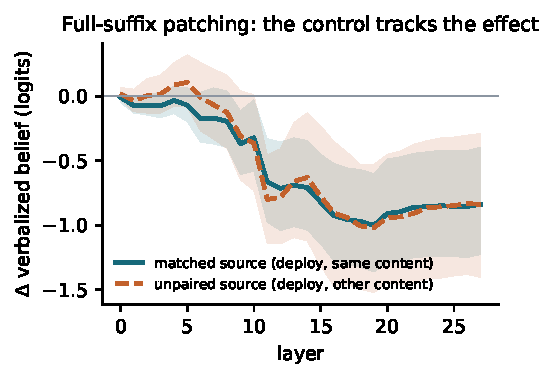
\includegraphics[width=\linewidth]{figures/pub_patch_layers.pdf}
\caption{The observation}
\end{subfigure}\hfill
\begin{subfigure}[t]{.48\linewidth}\centering
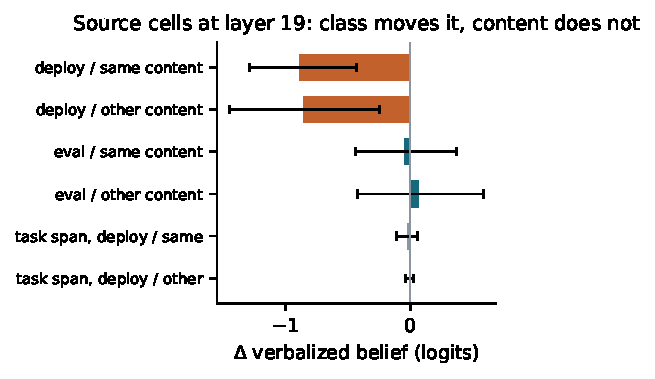
\includegraphics[width=\linewidth]{figures/pub_cells.pdf}
\caption{The diagnosis}
\end{subfigure}
\caption{(a) The unpaired control reproduces the matched patch effect
(Qwen2.5-1.5B; \NpairsExpTwo{} prompt pairs over \NclustersExpTwo{} held-out
content clusters; bands are content-clustered bootstrap CIs). (b) Completing
the source design to a 2$\times$2 of (class $\times$ content): both
deploy-class sources (top two bars) produce the effect and both eval-class
sources do not. My original contrast compared only the top two bars, and so
cancelled the class effect.}
\label{fig:exec}
\end{figure}

\textbf{The repaired analysis and the honest finding.} With all four source
cells, the estimated source-class effect at the readout span is
\NmeClass{} [\NmeClassLo{}, \NmeClassHi{}] logits; the content effect
(\NmeContent{} [\NmeContentLo{}, \NmeContentHi{}]) and the
class$\times$content interaction (\NixnMean{} [\NixnLo{}, \NixnHi{}]) are
not detectably different from zero. The class effect grows across
Qwen2.5-\{0.5B, 1.5B, 7B\} while the paired-minus-unpaired contrast stays
statistically indistinguishable from zero at every scale
(Table~\ref{tab:sensitivity}). Splitting the patched region finer shows what
the class signal is: on the primary model it is concentrated at the final
pre-answer position (\NEvalFinal{} [\NEvalFinalLo{}, \NEvalFinalHi{}];
reverse direction \NDeployFinal{} [\NDeployFinalLo{}, \NDeployFinalHi{}];
maximum-effect layer --- exploratory, locked analog in
Sec.~\ref{sec:confound}),
with the pre-question tokens contributing \NEvalTask{}
[\NEvalTaskLo{}, \NEvalTaskHi{}]. Across five models the pattern is
\emph{predominantly} report construction, with smaller but detectable
upstream transfer --- an order of magnitude below the final-position effect
--- at the question and pre-question tokens on the larger Qwen models
(Table~\ref{tab:position}). What patches move is mostly the state from which
the model is about to read out its answer, not evaluation-context processing
upstream of it. Both my original readings --- ``causal localization of
awareness'' and ``pure artifact'' --- were answers to a question my contrast
never asked.

\textbf{Strongest evidence against my interpretation.} (i) The class effect
could have reflected source--destination distance rather than class; a
matched design now bounds this --- with all four source cells at identical
per-position residual distance and only shrunk offsets, the effect stands at
\NmatchConMinEvalFinal{} [\NmatchConMinEvalFinalLo{},
\NmatchConMinEvalFinalHi{}] (Sec.~\ref{sec:confound}) --- though the
constructed estimand is the offset-direction effect at standardized dose,
not the raw class effect re-measured. (ii) Upstream transfer is
not absent: on Qwen-7B the question tokens carry $+0.24$ $[+0.11, +0.37]$ in
one direction and the same-content pre-question contrast is detectable in
both directions ($-0.10$ $[-0.18, -0.02]$ and $+0.16$ $[+0.06, +0.26]$),
and on the primary model the question tokens carry $-0.11$
$[-0.18, -0.04]$, so ``report construction'' is a predominance claim, not an
exclusivity claim. (iii) An all-layer
direction-ablation experiment was unstable under its own random control (the
control moved the outcome more than the treatment); I draw no conclusions
from it. (iv) A second-concept replication (register) was null on the primary model
and directional but not significant at 7B.

\textbf{Narrowest honest limitation.} One synthetic English corpus,
\NclustersExpTwo{} held-out content clusters, one readout question, models
$\le$8B; and the ``class transfer'' I localize is a property of a verbal
report --- I found no route from any of it to task behavior (sandbagging gaps
null or marginal on all five models).

\section{Setup, in brief}\label{sec:setup}
\textbf{Corpus and models.} \NContents{} task items rendered under five
evaluation and four deployment cue families (a no-lexicon exam family,
structurally matched metadata families, topic controls), split 50/50 into
train/test by content. Models: Qwen2.5-\{0.5B, 1.5B, 7B\}-Instruct,
Phi-3-mini-4k-instruct, Olmo-3-7B-Instruct (TransformerLens, Apple silicon);
primary model for in-text numbers: Qwen2.5-1.5B-Instruct in fp32. The
representational result of prior work reproduces here (held-out probe AUC
\NprobeAUC{}, permutation $p$ = \NpermP{}, computed at the selected layer and uncorrected for the max over layers (the permutation null's 95th percentile, 0.54 AUC, leaves any corrected version equally decisive); no-lexicon family transfer
\NsubtleAUC{}; topic-control false-positive rate \NtopicFPR{} against
\NevalRate{} for genuine evaluation framings) and I claim no novelty for it
\citep{nguyen2025probing,heidari2026evalaware,devbunova2026format}.

\textbf{Readout and direction.} The verbalized belief is a two-polarity
yes/no question appended after the task, scored from the first-answer-token
logits at the final input position (positive = ``I am being evaluated'');
$d_\ell = \mu^{\mathrm{eval}}_\ell - \mu^{\mathrm{deploy}}_\ell$
(unit-normalized), steering doses in units of $\sigma_\ell$. ``Final
pre-answer position'' below means that last input position: no answer token
has been generated when it is patched.

\textbf{Data accounting.} Layer sweeps: \NpairsExpTwo{} pairs over
\NclustersExpTwo{} content clusters; all CIs are content-clustered
bootstraps. Wherever a selected layer feeds a confirmatory estimate and that
layer was among those run, I report a locked version --- layer selected on a
discovery half of the clusters, effect re-estimated with a clustered
bootstrap on the other half (``locked''; 15 clusters each side; the one gap,
Phi-3, is named in \S\ref{sec:limits}); layers labeled maximum-effect were
selected on all data, and estimates at them are exploratory. \emph{Attrition and its repair:} an
earlier version of the 2$\times$2 required different-content sources to
share the readout span plus a two-token margin; on the Qwen and Olmo
tokenizers those sources share the readout span plus exactly one glue token,
so 34 of 60 candidate pairs were excluded (0 of 24 on Phi-3), leaving 13
clusters and model-dependent content subsets. The criterion was
tokenizer-determined and effect-blind (\texttt{results/attrition.json}), but
it made the models incomparable. All 2$\times$2 estimates reported here
therefore use one fixed list of the same \NclustersFone{} held-out contents
on every model, with the margin removed (readout span fully shared is the
only requirement). For different-content sources the content-specific pre-question tokens are
not shared by construction (only glue tokens and, for multiple-choice items,
the shared answer-format instruction survive the suffix match), so in the
tabulated pre-question column the two different-content cells are near-empty
patches and the 2$\times$2 main effect understates the same-content
pre-question contrast by roughly half (primary model: $-0.07$
$[-0.13, -0.01]$ same-content vs.\ \NEvalTask{} [\NEvalTaskLo{}, \NEvalTaskHi{}]
tabulated).

\section{The estimand mismatch}\label{sec:confound}
\textbf{What my contrast estimated.} Let $Y_{c,s}$ be the patch effect from
a source of class $c \in \{\mathrm{same}, \mathrm{other}\}$ relative to the
destination and content $s \in \{\mathrm{same}, \mathrm{other}\}$. The
matched patch is $Y_{\mathrm{other},\mathrm{same}}$; my unpaired control was
$Y_{\mathrm{other},\mathrm{other}}$. Their difference holds source class
fixed: it estimates the content-matching effect plus the class$\times$content
interaction and is structurally incapable of estimating a class effect. I
make no claim that the literature formally defines this contrast as a class
estimator; what I am reporting is the inference I made, which I believe is
tempting for anyone who reaches for an unrelated-prompt control
\citep{heimersheim2024patching,zhang2024bestpractices} --- read a large
matched effect as concept transfer, read a matching control as refutation
--- and which the design cannot license either way. It is distinct from
corruption-choice sensitivity \citep{zhang2024bestpractices} and from
subspace-patching illusions \citep{makelov2024illusion}; the nearest
analogue is over-control.

\textbf{The full factorial.} Adding the two same-class cells gives, at the
primary model's maximum-effect layer and readout span: estimated
source-class effect \NmeClass{} [\NmeClassLo{}, \NmeClassHi{}]; content
effect \NmeContent{} [\NmeContentLo{}, \NmeContentHi{}]; interaction
\NixnMean{} [\NixnLo{}, \NixnHi{}] (not detectable --- the condition under
which the simpler paired-minus-same-class contrast, \NReadContent{}
[\NReadContentLo{}, \NReadContentHi{}], is a clean class estimate). Because
that layer was chosen on all data, I also report a locked estimate: the
patch layer selected on the discovery half of the contents (layer
\NlockClassLayer{}, which coincides with the all-data choice), estimated on
the estimation-half contents only: \NlockClass{}
[\NlockClassLo{}, \NlockClassHi{}] (\NlockClassN{} clusters). Table~\ref{tab:sensitivity}
repeats the decomposition on five models: the class effect spans a wide
range while the paired-minus-unpaired contrast never leaves a
zero-straddling band. The class effect is depth-ordered ($\rho$ =
\NartifactDepthRho{}) and concentrates late --- the mismatch bites hardest
exactly where naive patching looks most impressive.

\begin{table}[t]\centering\small
\IfFileExists{tables/estimator_sensitivity.tex}{\begin{tabular}{lll}
\toprule
model & estimated source-class effect (2x2 CI) & paired-minus-unpaired contrast (CI) \\
\midrule
Qwen2.5-0.5B-Instruct & -0.32 [-0.47,-0.17] & +0.00 [-0.11,+0.11] \\
Qwen2.5-1.5B-Instruct & -1.09 [-1.29,-0.91] & +0.01 [-0.29,+0.29] \\
Qwen2.5-7B-Instruct & -2.37 [-2.94,-1.82] & -0.03 [-1.13,+1.14] \\
Phi-3-mini-4k-instruct & -0.29 [-0.39,-0.18] & +0.00 [-0.14,+0.15] \\
Olmo-3-7B-Instruct & -2.07 [-2.47,-1.69] & +0.02 [-0.91,+0.90] \\
\bottomrule
\end{tabular}
}{\todo{assets}}
\caption{The paired-minus-unpaired contrast does not respond to the estimated
source-class effect. Both columns: readout span at each model's
maximum-patch-effect layer (selected on all data --- exploratory; the locked
estimates are in Table~\ref{tab:landscape}), the same \NclustersFone{}
content clusters on every model, content-clustered bootstrap CIs.}
\label{tab:sensitivity}
\end{table}

\textbf{Where the class signal sits.} Splitting the patched region ---
pre-question task tokens, belief-question tokens, final pre-answer position
--- in both patch directions on all five models (Table~\ref{tab:position})
gives a predominance result, not an exclusivity result. On the primary model
the signal is concentrated at the final pre-answer position (\NEvalFinal{}
[\NEvalFinalLo{}, \NEvalFinalHi{}] vs.\ question
\NEvalQuestion{} [\NEvalQuestionLo{}, \NEvalQuestionHi{}] and pre-question
\NEvalTask{} [\NEvalTaskLo{}, \NEvalTaskHi{}]); the locked analog
(discovery-half layer, estimation-half clusters) gives \NlockFinalEval{}
[\NlockFinalEvalLo{}, \NlockFinalEvalHi{}] and, in the reverse direction,
\NlockFinalDeploy{} [\NlockFinalDeployLo{}, \NlockFinalDeployHi{}]; the locus differs by model
(question tokens on the smallest Qwen and on Olmo; final pre-answer position
on the larger Qwen models; every cell zero on Phi-3), and smaller upstream
transfer is detectable on the larger Qwen models --- always an order of
magnitude below the dominant position.
The interpretation I consider honest: patching mostly transplants the state
from which the model is about to read out its report --- constructed by the
final pre-answer position on larger Qwen models, still distributed over the
question tokens at 0.5B --- with a minority of transfer that is genuinely
upstream. Olmo also splits the region in a way that explains its steering
anomaly (\S\ref{sec:landscape}): large normal-signed transfer at the
question tokens and, in one patch direction, sign-inverted transfer at the
final pre-answer position, so instruments that weight positions differently
must disagree.

\begin{table}[t]\centering\footnotesize
\IfFileExists{tables/position_models.tex}{\begin{tabular}{lllll}
\toprule
model & destination & pre-question & question & final pre-answer \\
\midrule
Qwen2.5-0.5B-Instruct & eval dest. & -0.00 [-0.00,+0.00] & -0.01 [-0.01,-0.00] & -0.34 [-0.49,-0.20] \\
Qwen2.5-0.5B-Instruct & deploy dest. & +0.00 [-0.00,+0.00] & +0.01 [-0.00,+0.01] & +0.37 [+0.23,+0.50] \\
Qwen2.5-1.5B-Instruct & eval dest. & +0.00 [-0.00,+0.00] & -0.19 [-0.24,-0.15] & -0.89 [-1.07,-0.73] \\
Qwen2.5-1.5B-Instruct & deploy dest. & +0.00 [-0.00,+0.01] & +0.26 [+0.21,+0.30] & +1.07 [+0.88,+1.27] \\
Qwen2.5-7B-Instruct & eval dest. & +0.04 [+0.00,+0.07] & +0.19 [+0.11,+0.27] & -2.55 [-3.11,-1.98] \\
Qwen2.5-7B-Instruct & deploy dest. & +0.01 [-0.02,+0.03] & -0.17 [-0.26,-0.10] & +3.14 [+2.51,+3.77] \\
Phi-3-mini-4k-instruct & eval dest. & +0.00 [-0.00,+0.01] & -0.01 [-0.02,-0.00] & -0.29 [-0.40,-0.19] \\
Phi-3-mini-4k-instruct & deploy dest. & -0.00 [-0.01,+0.00] & +0.00 [-0.00,+0.01] & +0.44 [+0.32,+0.56] \\
Olmo-3-7B-Instruct & eval dest. & +0.01 [-0.02,+0.04] & -1.60 [-1.85,-1.34] & -0.47 [-0.62,-0.32] \\
Olmo-3-7B-Instruct & deploy dest. & +0.05 [+0.01,+0.08] & +1.84 [+1.56,+2.12] & +0.54 [+0.39,+0.69] \\
\bottomrule
\end{tabular}
}{\todo{assets}}
\caption{Estimated source-class effect by patched position, both patch
directions, all five models (maximum-effect layer, selected on all data ---
exploratory; locked final-position analogs in the text; the same \NclustersTen{}
content clusters per row on every model; content-clustered CIs).}
\label{tab:position}
\end{table}

\textbf{Distance is matched by construction.} Per-cell source--destination
residual distances were recorded for every patch, and observationally they
cut against a distance account (the inert same-class/different-content
source lies \emph{farther}, $\ell_2$ = \NdistSameDiff{}, than the potent
other-class/same-content source, \NdistPaired{}). Because that is a check
and not a design, I re-ran the full 2$\times$2 with distance handled by
construction (Experiment J): same destinations, patched spans equalized
across the four cells, same clustered estimator, \NmatchClusters{} clusters
per destination class (unmatched baseline under this discipline:
\NmatchUnEvalFinal{} [\NmatchUnEvalFinalLo{}, \NmatchUnEvalFinalHi{}] /
\NmatchUnDeployFinal{} [\NmatchUnDeployFinalLo{}, \NmatchUnDeployFinalHi{}],
reproducing the published estimates). Distances are functions of activations
fixed before any intervention, so matching on them is outcome-blind
covariate matching; exact balance among \emph{real} activations is
nevertheless geometrically impossible if class is linearly encoded (an
other-class source has a distance floor), so selection serves as the
on-manifold check and construction as the primary instrument.
\emph{Distance-selected} (best of \NmatchK{} candidate renderings per cell,
chosen --- before any effect is computed --- to zero the class-condition
distance gap; achieved gap \NmatchSelGapEval{} vs.\ \NmatchUnGapEval{}
unmatched, eval destinations): class effect \NmatchSelEvalFinal{}
[\NmatchSelEvalFinalLo{}, \NmatchSelEvalFinalHi{}] /
\NmatchSelDeployFinal{} [\NmatchSelDeployFinalLo{},
\NmatchSelDeployFinalHi{}]. \emph{Distance-constructed} (each source's
per-position offset rescaled to the four-cell mean norm, so all four cells
sit at identical $\ell_2$ distance at every patched position; mean rescale
\NmatchScale{}): \NmatchConEvalFinal{} [\NmatchConEvalFinalLo{},
\NmatchConEvalFinalHi{}] / \NmatchConDeployFinal{}
[\NmatchConDeployFinalLo{}, \NmatchConDeployFinalHi{}].
\emph{Shrink-only construction} (rescale to the four-cell \emph{minimum}
norm: every patched state is a convex interpolation toward the destination,
no offset is ever amplified, so rescaling can only attenuate whatever the
offset carries --- the conservative primary, decision rule committed before
the runs): \NmatchConMinEvalFinal{} [\NmatchConMinEvalFinalLo{},
\NmatchConMinEvalFinalHi{}] / \NmatchConMinDeployFinal{}
[\NmatchConMinDeployFinalLo{}, \NmatchConMinDeployFinalHi{}]. The locked
versions (discovery-half layer \NmatchLockLayer{}, estimation-half
clusters, $n$ = \NmatchLockConMinN{}) stand: shrink-only \NmatchLockConMin{}
[\NmatchLockConMinLo{}, \NmatchLockConMinHi{}], selected \NmatchLockSel{}
[\NmatchLockSelLo{}, \NmatchLockSelHi{}]. Balance also holds in a
unit-direction metric (matched-arm class-condition gaps below $0.005$ in
every cell on every model and $\le 0.003$ at the final position; $0.002$ and
$0.001$ on the primary model), so RMSNorm radial
invariance does not hide an imbalance, and the rescale footprint --- the
paired unmatched-minus-constructed change in each cell's own effect ---
stays within $0.59$ logits across all cells, spans and layers on the
primary model ($0.53$ at the final position) and within $1.85$ logits on any
of the five, bounding what off-manifold distortion could contribute. Two scope notes: the
constructed arms estimate the effect of the class-associated offset
\emph{direction} at standardized per-position dose (equalizing magnitude
removes any magnitude-mediated share of the raw effect along with the
confounded share), and the selected arm re-matches per analysis cell; all
arms share one survivor set of destinations, and the constructed arms reuse
the unmatched sources. At matched --- and at identical --- residual
distance, class still orders the effect (Table~\ref{tab:matched}). On the two
models whose final-position class effect is detectable in \emph{both} patch
directions the shrink-only estimate attenuates relative to the unmatched one (1.5B $-0.82
\rightarrow -0.62$; 7B $-2.27 \rightarrow -1.26$) while excluding zero in
both patch directions: part of the raw effect does travel with offset
magnitude, and the majority does not. The result is not confined to that
position. Qwen2.5-0.5B carries no final-position effect to match --- its
locus is the belief-question span (\S\ref{sec:confound},
Table~\ref{tab:position}) --- and matched over the readout span that
contains that locus it replicates too: shrink-only $-0.25$ $[-0.32, -0.18]$
and, in the reverse direction, $+0.15$ $[+0.09, +0.22]$ (Experiment J
resolves final, readout and pre-question spans, not the question tokens
alone). Table~\ref{tab:matched} therefore carries a
readout-span column, so a model whose class effect does not sit at the
final position is not represented by a row of zeros.

\textbf{Where matching removes an effect.} Olmo-3-7B is the case the matched
design argues against itself, and it is worth stating plainly. Its
anomalous \emph{sign-inverted} final-position effect --- the one that
mechanically explains its inverted steering (\S\ref{sec:landscape}) --- does
not survive the conservative arm: unmatched $-0.50$ $[-0.91, -0.09]$
(deploy destinations) becomes $-0.34$ $[-0.59, -0.09]$ when matched by
selection, $-0.38$ $[-0.75, -0.00]$ when constructed, and $-0.07$
$[-0.25, +0.11]$ under shrink-only construction, which no longer excludes
zero. I read that inversion as partly a magnitude phenomenon rather than
class transfer, and I do not claim it as a matched result. What does survive
on Olmo is the effect at its own locus, the belief-question tokens, and it
survives \emph{normal}-signed in both directions (shrink-only $-0.39$
$[-0.61, -0.15]$ and $+0.53$ $[+0.27, +0.81]$ over the readout span). Phi-3-mini,
which has no detectable class effect anywhere in the unmatched design, has
none under matching either: every arm, span and direction stays within
$0.01$ logits of zero at the maximum-effect layer and $0.04$ at every layer
run --- a calibration check on the instrument rather than
a replication. The pre-question task span stays
\emph{small} under matching on all five models --- every matched estimate at
the maximum-effect layer lies within $0.05$ logits of zero (largest,
Qwen-7B shrink-only deploy destinations, $-0.05$ $[-0.09, -0.01]$) --- but
several of those small values do exclude zero, so this reproduces the
predominance claim of \S\ref{sec:confound} under matching, not an
exclusivity claim. All five checkpoints have now completed Experiment
J on the same \NmatchClusters{} content clusters per destination class.

\begin{table}[t]\centering\footnotesize
\IfFileExists{tables/matched_models.tex}{\begin{tabular}{lllllll}
\toprule
model & destination & unmatched & distance-selected & distance-constructed & shrink-constructed & shrink, readout span \\
\midrule
Qwen2.5-0.5B-Instruct & eval dest. & -0.34 [-0.49,-0.20] & -0.26 [-0.44,-0.10] & -0.39 [-0.54,-0.24] & -0.28 [-0.39,-0.17] & -0.28 [-0.40,-0.18] \\
Qwen2.5-0.5B-Instruct & deploy dest. & +0.37 [+0.23,+0.50] & +0.17 [+0.04,+0.33] & +0.34 [+0.22,+0.48] & +0.19 [+0.12,+0.26] & +0.19 [+0.13,+0.26] \\
Qwen2.5-1.5B-Instruct & eval dest. & -0.89 [-1.07,-0.73] & -0.61 [-0.78,-0.46] & -0.81 [-0.97,-0.67] & -0.59 [-0.70,-0.49] & -0.72 [-0.86,-0.60] \\
Qwen2.5-1.5B-Instruct & deploy dest. & +1.07 [+0.88,+1.27] & +0.46 [+0.36,+0.56] & +0.79 [+0.62,+0.96] & +0.44 [+0.34,+0.54] & +0.54 [+0.42,+0.65] \\
Qwen2.5-7B-Instruct & eval dest. & -2.55 [-3.11,-1.98] & -1.51 [-2.01,-1.00] & -2.19 [-2.71,-1.65] & -1.55 [-1.95,-1.16] & -1.39 [-1.78,-1.00] \\
Qwen2.5-7B-Instruct & deploy dest. & +3.14 [+2.51,+3.77] & +1.87 [+1.43,+2.33] & +2.42 [+1.83,+3.04] & +1.38 [+1.03,+1.73] & +1.25 [+0.91,+1.58] \\
Phi-3-mini-4k-instruct & eval dest. & -0.29 [-0.40,-0.19] & -0.24 [-0.36,-0.14] & -0.23 [-0.33,-0.14] & -0.16 [-0.23,-0.09] & -0.16 [-0.24,-0.09] \\
Phi-3-mini-4k-instruct & deploy dest. & +0.44 [+0.32,+0.56] & +0.28 [+0.19,+0.38] & +0.39 [+0.28,+0.51] & +0.26 [+0.18,+0.35] & +0.26 [+0.18,+0.35] \\
Olmo-3-7B-Instruct & eval dest. & -0.47 [-0.62,-0.32] & -0.40 [-0.53,-0.29] & -0.42 [-0.59,-0.24] & -0.28 [-0.38,-0.18] & -1.44 [-1.75,-1.15] \\
Olmo-3-7B-Instruct & deploy dest. & +0.54 [+0.39,+0.69] & +0.32 [+0.20,+0.44] & +0.49 [+0.33,+0.65] & +0.29 [+0.20,+0.37] & +1.35 [+1.12,+1.58] \\
\bottomrule
\end{tabular}
}{\todo{assets}}
\caption{Distance-matched estimated source-class effects, both patch
directions, for every model with a completed Experiment J run. The four estimate columns
after the destination are the final pre-answer position; the last is the
shrink-only estimate over the whole readout span (belief question $+$ final position),
which contains every model's locus and so remains informative for models
whose class effect does not sit at the final position. Maximum-effect layer
--- exploratory; the locked shrink-only estimate is in the text;
content-clustered CIs.}
\label{tab:matched}
\end{table}

\textbf{Scope.} The same 2$\times$2 on a second concept (register, formality
readout) gave a null class effect at 1.5B ($-0.08$ $[-0.45, +0.25]$) and a
directional but non-significant one at 7B ($-0.41$ $[-1.09, +0.26]$; 12
contents), so the estimand point generalizes by its logic --- a contrast
that fixes the concept label cannot estimate that label's effect --- rather
than by a second demonstrated instance.

\section{Convergent evidence from steering}\label{sec:steering}
Steering $\pm\alpha\sigma_\ell\hat d_\ell$ transplants no span. Held to a
pre-specified battery --- a locked layer (selected on the discovery split;
on the primary model it coincides with the all-data steering peak, at which
the dose and percentile diagnostics below are computed), dense
dose-response, distributional checks (KL from the unsteered next-token
distribution at every dose), and a null of 100 matched-norm random directions
over \NclustersReg{} clusters --- steering on the primary model moves the
verbalized belief at the locked layer by \NlockSteerEval{}
[\NlockSteerEvalLo{}, \NlockSteerEvalHi{}] (eval framing) and
\NlockSteerDeploy{} [\NlockSteerDeployLo{}, \NlockSteerDeployHi{}] (deploy
framing). I treat the low-KL regime ($|\alpha| \le 1$, KL $\le$
\NdoseKLsmall{} nats) as primary: there the swing is \NswDsmall{}
[\NswDsmallLo{}, \NswDsmallHi{}] and $|d|$ sits at the \NpctSmall{}th
percentile of the random-direction null (Fig.~\ref{fig:steer}a). Large
doses (mean KL \NdoseKLbig{} nats at $|\alpha| = 8$, averaged over framings)
are reported as secondary. Steering and
the repaired patching estimator agree in sign and rough magnitude on the
Qwen family --- convergent evidence that the class variable is real and
manipulable --- while remaining, like patching, interventions on what the
model \emph{reports}: none of them measurably changed task behavior
(\S\ref{sec:landscape}).

\begin{figure}[t]\centering
\begin{subfigure}[t]{.48\linewidth}\centering
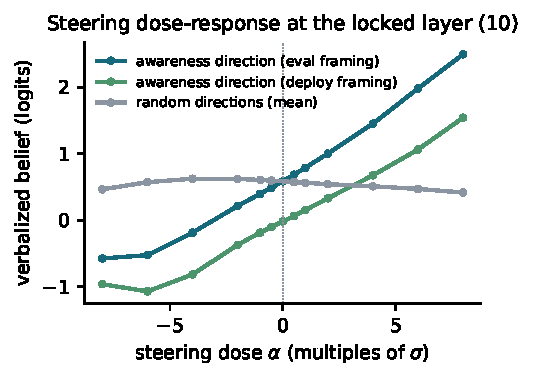
\includegraphics[width=\linewidth]{figures/pub_dose.pdf}
\caption{Dose-response at the locked layer}
\end{subfigure}\hfill
\begin{subfigure}[t]{.48\linewidth}\centering
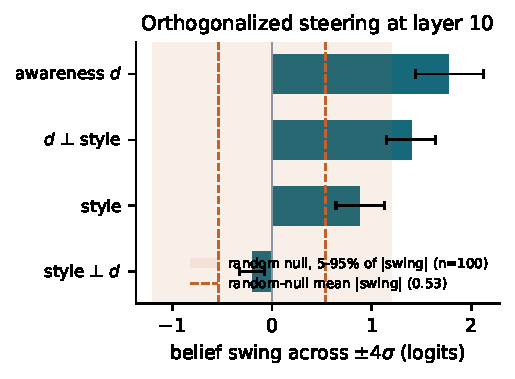
\includegraphics[width=\linewidth]{figures/pub_register.pdf}
\caption{Orthogonalized steering vs.\ the random null}
\end{subfigure}
\caption{(a) Steering dose-response at the locked layer; random-direction
mean for comparison. (b) Matched-norm swings for the awareness direction, the
style direction, and each orthogonalized to the other, against the
5--95\% band of $|$swing$|$ over 100 random directions (secondary result,
\S\ref{sec:register}).}
\label{fig:steer}
\end{figure}

\section{Instrument validity across five models}\label{sec:landscape}
\begin{table}[t]\centering\footnotesize
\setlength{\tabcolsep}{3pt}
\resizebox{\linewidth}{!}{%
\IfFileExists{tables/cross_model.tex}{\begin{tabular}{lrrllll}
\toprule
model & probe AUC & verbal AUC & sandbag gap (paired CI) & locked steering (eval framing) & class effect, max-effect layer (exploratory) & class effect, locked (disc.-half layer, est.-half contents) \\
\midrule
Qwen2.5-0.5B-Instruct & 0.967 & 0.818 & +0.03 [-0.06,+0.14] & L9: -0.63 [-0.68,-0.58] & -0.32 [-0.47,-0.17] (n=30) & -0.26 [-0.51,-0.07] (n=15) \\
Qwen2.5-1.5B-Instruct & 0.956 & 0.942 & +0.02 [-0.10,+0.15] & L10: -0.41 [-0.48,-0.33] & -1.09 [-1.29,-0.91] (n=30) & -1.19 [-1.45,-0.94] (n=15) \\
Qwen2.5-7B-Instruct & 0.977 & 0.937 & -0.00 [-0.03,+0.03] & L12: -3.05 [-3.20,-2.88] & -2.37 [-2.94,-1.82] (n=30) & -2.83 [-3.58,-2.13] (n=15) \\
Phi-3-mini-4k-instruct & 0.981 & 0.899 & +0.01 [-0.04,+0.08] & L16: +0.34 [+0.32,+0.36] & -0.29 [-0.39,-0.18] (n=30) & -0.30 [-0.46,-0.14] (n=15) \\
Olmo-3-7B-Instruct & 0.994 & 0.851 & +0.05 [-0.00,+0.13] & L8: -0.75 [-0.85,-0.66] & -2.07 [-2.47,-1.69] (n=30) & -2.04 [-2.75,-1.36] (n=15) \\
\bottomrule
\end{tabular}
}{\todo{assets}}}
\caption{Five models, identical instruments and identical content clusters.
``Locked steering'': held-out eval-framing estimate at the discovery-selected
layer. Class effects: the 2$\times$2 estimate at the readout span, at the
all-data maximum-effect layer (exploratory) and locked (layer selected on the
discovery half of contents, estimated on the other half). Sandbagging CIs are paired and
content-clustered ($n$ = \NsandbagNitems{} items per model).}
\label{tab:landscape}
\end{table}

The encoding side is consistent everywhere (probe AUC 0.956--0.994 with
format controls passing; the readout region dominates causal span maps in
all five). The causal side is not. On Qwen, locked steering grows with scale
($-0.29 \to -0.84 \to -2.20$) and the source-class effect grows with it. On
Phi-3-mini nothing meaningfully moves the report: the largest eval-framing
steering effect at any layer is $-0.030$ $[-0.044, -0.016]$ (deploy framing
$+0.036$ $[+0.025, +0.049]$) --- two orders of magnitude below Qwen-7B ---
and every 2$\times$2 cell is zero. On Olmo-3-7B, locked steering CIs exclude
zero ($+0.32$ $[+0.12, +0.53]$ eval framing) with \emph{inverted} signs, and
orthogonalized steering shows $d$, style, and random directions all moving
the readout comparably --- the inverted-steering regime of
\citet{torop2026inverted}, arising in the wild; effect-size-with-CI
reporting would have passed it as replication. The positional split of
\S\ref{sec:confound} explains the configuration (question tokens normal,
final pre-answer position inverted in one direction), and the 2$\times$2
still detects class transfer on Olmo. Instruments dissociate on the same model; that is the
strongest argument I know for running all of them.

Behavior, for context and consistent with prior work
\citep{knecht2026limited,li2026decomposing}: incentivized sandbagging gaps
are null with bounded CIs on four models (Qwen-7B: $-0.00$
$[-0.03, +0.03]$; pooled Qwen: \NpooledGap{}
[\NpooledGapLo{}, \NpooledGapHi{}]) and marginal on Olmo ($+0.054$
$[-0.002, +0.126]$); steering the belief direction hard enough to move the
report by a logit moves accuracy by \NswingDAcc{}.

\section{Secondary result: the register share of the steerable signal}\label{sec:register}
A style direction --- the mass-mean of formal-vs-casual framings, built
from deployment-side prompts only --- is substantially aligned with $d$ in
every model ($\cos$ = 0.46--0.68 at the steering layer). Steering with $d$,
style, and each orthogonalized to the other at matched norm
(Fig.~\ref{fig:steer}b) shows the style axis going from causally inert at
0.5B (2\% of $d$'s swing; $d_{\perp\mathrm{style}}$ keeps 97\%) to parity
with $d$ at 7B (64\% of $d$ surviving orthogonalization; in the low-KL
regime on the primary model, \NfracDperpSmall{}). I report this as a
within-family trend with caveats, not a scaling law: three sizes of one
family; a style direction constructed from my own deployment framings, which
is \emph{correlated with}, not guaranteed free of, evaluation-context
information; and a random-direction floor that is a substantial fraction of
$d$'s swing at small scale. Its value is as a causal-level counterpart to
the probe-level format-sensitivity critique \citep{devbunova2026format}:
belief-report controllability claims need register controls.

\section{Related work}
Evaluation awareness: decodability, steering, scaling, and dissociations
\citep{needham2025evaluated,nguyen2025probing,abdelnabi2025linear,heidari2026evalaware,hua2026steering,chaudhary2025scaling,manek2026depth,nayan2026notone,knecht2026limited,li2026decomposing};
format-sensitivity of probes \citep{devbunova2026format}. Patching
methodology: corruption-type sensitivity \citep{zhang2024bestpractices},
practice \citep{heimersheim2024patching,wang2022ioi}, subspace illusions
\citep{makelov2024illusion}; the estimand of the control contrast is
orthogonal to all three. Steering validity: inverted steering vectors
\citep{torop2026inverted}; steering practice
\citep{zou2023repe,turner2023activation,rimsky2023caa,arditi2024refusal}.

\section{Limitations, and evidence against}\label{sec:limits}
Report-construction predominance is a predominance claim: upstream transfer
is detectable at the question and pre-question tokens on the larger Qwen
models, an order of magnitude below the dominant position. Content and interaction
``nulls'' are bounded, not negligible: a TOST-style equivalence analysis
(90\% clustered bootstrap CIs; final position, maximum-effect layer;
\texttt{scripts/equivalence\_bounds.py}) bounds the primary model's content
and interaction effects within 0.42--0.63 logits, i.e.\ 0.51--0.72$\times$
the class effect (both destinations), with 0.47--0.75$\times$ on Qwen-7B
deploy destinations; on Olmo, and wherever the final-position class effect
is itself undetectable, no informative equivalence claim is supportable.
One cell is not a null at all: the Qwen-7B eval-destination interaction at
the final position is detectably positive ($+1.93$ $[+0.35, +3.68]$, 95\%),
so the same-content class contrast there is weaker than the
different-content one. The maximum-effect layer was selected on all data; the locked estimates
(discovery-half layer, estimation-half contents) agree but use 15 clusters,
and are not computable for Phi-3 (whose discovery-selected layer was not
among those run). An all-layer direction-ablation
experiment was unstable under its own random control (control \NmlRdsep{}
[\NmlRdsepLo{}, \NmlRdsepHi{}], treatment \NmlDdsep{}
[\NmlDdsepLo{}, \NmlDdsepHi{}], not distinguishable from zero) and is
excluded from all claims. The register replication did not reach
significance. Behavioral nulls are bounded by 24-item suites. One corpus,
synthetic, English; five models $\le$8B from three labs.

\section{Disclosure and verification}\label{sec:disclosure}
\textbf{Tools.} Code, experiment orchestration, and drafting were done with
substantial assistance from Anthropic's Claude (Claude Code); the framing of
the estimand critique and the list of blocking issues addressed in this
version came from written critiques produced with OpenAI's ChatGPT/Codex.
Multi-agent LLM audits cross-checked prose against result files; the errors
they found are corrected here, and I do not treat them as a substitute for
the personal verification below.

\textbf{What I personally designed, read, and checked.}
\tofill{which hypotheses and controls you designed yourself (e.g.\ the
2$\times$2 completion, the locked split, the positional split)}.
\tofill{which code paths you read end to end (e.g.\ patching hooks in
\texttt{interventions.py} and \texttt{exp7}/\texttt{exp10}; the belief
readout in \texttt{readouts.py})}.
\tofill{how many raw prompts and readouts you inspected by hand
(\texttt{scripts/sample\_audit.py}), and whether alignments and scores looked
right}.
\tofill{which headline numbers you independently recomputed from the CSVs
(e.g.\ the class main effect, the interaction, one locked steering CI)}.
\tofill{what remains unchecked}.
\tofill{for each component --- corpus, patching, steering, statistics --- how
surprised you would be by a major error, in one line each}.
\tofill{total active hours, and a short decision timeline}.
\tofill{exact contribution of anyone else who participated, or ``none''}.

\bibliographystyle{plainnat}
\bibliography{references}

\end{document}
